\documentclass[11pt,titlepage,a4paper]{article}
%%% Preamble %%%

% Packages: I comment ones I don't need or am not using to cut down on compiling time.

	% Default: AMS maths packages

		\usepackage{amsmath}
		\usepackage{amssymb}
		\usepackage{amsfonts}
		\usepackage{mathtools} % Fixes bugs with the ams packages and provides additional functionality.

	% Geometry: The layout of the document.

		\usepackage[width = 15 cm, left = 3 cm, height = 23 cm, top = 3 cm]{geometry} % A4 Paper, W = 21 cm, H = 29.7 cm. Paper width = left + width + right, Paper length = top + height + bottom.

	% 	\usepackage{multicol} % Used to switch to two column mode.
	% 	\setlength{\columnsep}{0.75cm} % Determines the length between columns

	% Graphics: Allows images.

		\usepackage{graphicx} % Used to include images.
	% 	\usepackage{float} % For figures in multicolumn
	% 	\usepackage{wrapfig} % Used to have multiple figures in a single beamer slide.

		\graphicspath{./Figures/} % The location of figures used in this document. Trailing / required.

	% Diagrams: Diagram creation.

		\usepackage{tikz} % Creates diagrams, needs calc for arithmetic.
		\usepackage{calc}

	% Figures: Extends figure functionality, allows multiple figures per float environment.

		\usepackage[singlelinecheck=off]{caption} % Needed for subcaption. Adds functionality to all captions. Single line check option needed to left align long table captions.
	%	\usepackage{subcaption} % Allows creation of subfigures, which allows multiple labelled figures per environment.

	% Tables: Extends table functionality, allows multiple page tables.

		\usepackage{booktabs} % Enhances tables with additional functionality.
		\usepackage{longtable} % Allows tables to extend to more than one page.
		\usepackage{multirow} % Allows cells to stretch over multiple rows like multicolumn.

	% Titles: Modifies titles, especially for multicolumns

	% 	\usepackage{titlesec}

	% 	\titleformat{\section}
	% 		{\normalfont\Large\bfseries\centering}
	% 		{\thesection}{1ex}{}

	% 	\titleformat{\subsection}
	% 		{\normalfont\large\bfseries\centering}
	% 		{\thesubsection}{1ex}{}

	% Theorems: Defines theorems, axioms, definitions, etc in a custom environment.

	%\usepackage{amsthm} % Needed for the definitions

	%	%This style is in italics and can be used as a subsection
	%	\newtheoremstyle{conditionStyle}% Name
	%		{3pt}% Space above
	%		{3pt}% Space below
	%		{}% Body font
	%		{\parindent}% Indent amount
	%		{\itshape}% Theorem ead font
	%		{:}% Punctuation after theorem ead
	%		{.5em}% Space after theorem ead
	%		{}% Theorem head spec (can be left empty, meaning `normal')

	%	\newtheoremstyle{solutionStyle}% name of the style to be used
	%		{3pt}% measure of space to leave above the theorem. E.g.: 3pt
	%		{3pt}% measure of space to leave below the theorem. E.g.: 3pt
	%		{}% name of font to use in the body of the theorem
	%		{}% measure of space to indent
	%		{\bfseries}% name of head font
	%		{:}% punctuation between head and body
	%		{.5em}% space after theorem head; " " = normal interword space
	%		{}% Manually specify head

	%	\newtheorem{axiom}{Axiom}
	%	\newtheorem{property}{Property}
	%	\newtheorem{rl}{Rule}
	%	\newtheorem{law}{Law}		
	%	\newtheorem{thm}{Theorem}
	%	\newtheorem{ex}{Example}
	%	\newtheorem{prn}{Principle}
	%	\newtheorem{prf}{Proof}
	%	\newtheorem{lma}{Lemma}

	%	\theoremstyle{definition}
	%	\newtheorem{exc}{Excercise}
	%	\newtheorem{defn}{Definition}
	%	\newtheorem{clm}{Claim}

	%	\newtheorem{qst1}{Question}
	%	\newtheorem{qst}{Question}[qst1]
	%	\newtheorem{sol1}{Solution}
	%	\newtheorem{sol}{Solution}[sol1]

	%	\theoremstyle{conditionStyle}
	%	\newtheorem{condition}{Condition}[rl]

	% Utility: Packages that add extra functionality.

	% 	\usepackage{xcolor} % Used to make footnote numbering red.
	% 	\usepackage{esdiff} %easy differentials eg. \diff[n]{y}{x}, \diffp[n]{y}{x}.
		\usepackage{verbatim} % Used to write code.
	%	\usepackage{textcomp} % Provides roman greek letters.
	% 	\usepackage{eurosym} % Provides accurate euro symbol.
	% 	\usepackage{enumerate} % Needed for lists that use lower case roman numerals.
		\usepackage{xfrac} % used for inline fractions (e.g. a/b via \sfrac{a}{b}).
		\usepackage{thmtools}

	% Editing: Packages and settings used to make papers easier to edit and to test output.

	%	\usepackage{lipsum} % Generates Lorem Ipsum.
	%	\usepackage[pagewise]{lineno} % Used for editing to add line numbers to the left hand side. Use \linenumbers to beging and \nolinenumbers to turn off.

	%	\linespread{1.6} % This changes the the line spacing. A line spacing factor of 1.3 is equivalent to one and a half line spacing and 1.6 is equal to double line spacing.

	% Datetime: Changes the date.

		\usepackage[UKenglish]{isodate}% Used to change the date format.
		\cleanlookdateon % Removes the ordinal suffix

	% Custom accents

	% \usepackage{accents}
	
	% \newlength{\dtildeheight}
	% \newcommand{\doubletilde}[1]{%
	%     \settoheight{\dtildeheight}{\ensuremath{\tilde{#1}}}%
	%     \addtolength{\dtildeheight}{-0.35ex}%
	%     \tilde{\vphantom{\rule{1pt}{\dtildeheight}}%
	%     \smash{\tilde{#1}}}}

	% BibLaTeX: The citestyles and bib file used in citations are edited here.

		\usepackage[backend=biber,citestyle=numeric-comp,doi=true,url=true]{biblatex} % Additional functionality for bibtex, use sorting=none to order in terms of appearance rather than alphabetically.
		\addbibresource{Bibliography.bib}

		\usepackage[utf8]{inputenc} % Allows unicode, so that umlauts will appear in the bibliography

	% Microtyping: The microtype package has several options that affect the way the document is compiled, these go here.

		\usepackage[final,tracking=true,kerning=true,spacing=true]{microtype}
		\microtypecontext{spacing=nonfrench}

	% Referencing: All the referencing packages tend to be loaded last to avoid problems. Order is hyperref then cleveref.

		\usepackage[colorlinks=false,pdfborder={0 0 0},citecolor=blue,urlcolor=blue]{hyperref} % Makes all labels hyperlinks, minus the ugly border.
		\usepackage[noabbrev]{cleveref} % Cleveref has made all the time I spent making reference completions redundant, thanks cleveref.

% Command Creation: I comment out the ones I don't need, but keep them as templates for future commands.

	% Big-O notation
	\newcommand{\BigO}[1]{\ensuremath{\operatorname{O}\left(#1\right)}}

	% \renewcommand\thefootnote{\textcolor{red}{\arabic{footnote}}} % Will make the indecies used in footnotes red to keep in line with the documents colour scheme.

	% \newcommand{\degrees}{\, ^{\circ}\mathrm{C}}

	% For tables in multicolumn.

	% \makeatletter
	% 	\newenvironment{tableplease}
	% 	  {\def\@captype{table}}
	% 	  {}
 	%  	\makeatother

 	%  	For centering tables in multicolumn, eliminates unwanted vertical space.

	% \newenvironment{tightcenter}{%
	%  \setlength\topsep{0pt}
	%  \setlength\parskip{0pt}
	%  \begin{center}
	% }{%
	%  \end{center}
	% }

	% Custom Counter Numbering

	% \numberwithin{equation}{qsol} % Equation numbers will follow the numbering scheme of qsol.

% Math operators declaration

	\DeclareMathOperator\erf{erf}

	\usepackage[parfill]{parskip}

% Document Structure

	\setcounter{secnumdepth}{3}

% Title: The title that appears in the report is edited here.

	\title{\textbf{Random Walks for Modelling Cell Populations} \\ VRES 2013-14}
	\author{\textbf{Morgan Wall} \\ n7532962}
	\date{\today}

%%% Document %%%

\begin{document}

%%% Title %%%

\maketitle

%%% Abstract %%%

% \begin{abstract}

%	\noindent 

% \end{abstract}

%%% Contents page %%%

\tableofcontents
\pagebreak

%%% Body %%%

\section{Introduction}
	\label{sec:introduction}
	
	This report documents the tasks completed by Morgan Wall as part of his 2013-14 VRES scholarship with Dr. Matthew Simpson. The project covered the use of random walks in simulating cell motility, proliferation, and interaction in a variety of biological contexts. Furthermore, the derivation and analysis of partial differential equations (PDEs) to model equivalent processes was considered.

% end sec:introduction

\section{Simulating Random Walks in 2D}
	\label{sec:simrandin2d}
	
	Mathematically, random walks consist of a sequence of numbers generated independently via stochastic processes \cite{grinstead1997}. Random walks can be used in modelling a wide variety of physical phenomenon. Several biological random walk models, either analsyed or proposed by Simpson, were researched. Each model accounted for cell motility and proliferation, which describes a cell's ability to move spontaneously and cell mitosis, respectively. Both of these cellular mechanisms are essential in modelling the biological processes considered \cite{simpson2009diffusing,simpson2010cell}. The models varied based on the consideration of cell interactions via volume exclusion or by the proliferation mechanism used.

	\subsection{Methodology}
		\label{sub:methodology}
		
		There exists several methods for visualising a random walk \cite{grinstead1997}. This research project focused on constraining the random walk to a multi-dimensional rectangular lattice. The methodology applied mimics that of Simpson's prior work \cite{simpson2009diffusing,simpson2010cell}. Considering a two-dimensional $m \times n$ lattice, for example, agents can assume positions at $(i, j)$, where $i, j \in \mathbb{N^+}$, $i \le m$, and $j \le n$. Each non-boundary node $(i, j)$ therefore has the neighbouring nodes: $(i, j + 1)$, $(i, j - 1)$, $(i + 1, j)$, and $(i - 1, j)$. Typically, a combination of periodic \cite{periodiccond} and reflective boundary conditions \cite{reflectivecond} are imposed on the lattice. 

		The sequence of random numbers generated for a random walk were used in moving agents, initially positioned on the lattice, to neighbouring nodes. Furthermore, such random numbers may also have been used for placing daughter agents at an adjacent node in replicating cell mitosis. Over a period of time, such movement would form a path taken by an agent in discrete, random steps. For simulations, time was consequently discretised into fixed time steps of duration $\delta t$. Following Simpson's approach, given that $N$ agents are present at the start of a time step, $N$ agents were selected at random for action. Depending on the biological process being modelled, each action could include both motility and proliferation events. The exact algorithms constituting an action are defined in detail in \cite{simpson2009diffusing,simpson2010cell} and for brevity they are not redefined in this report.
	
	% end sub:methodology

	\subsection{Implementation}
		\label{sub:implementation}
		
		The random walk models defined in \cite{simpson2009diffusing,simpson2010cell} were reproduced using the C programming language in conjunction with Intel's Math Kernel Libraries (MKL). The results of all simulations were output to CSV files for analysis and visualisation using MALTAB. A substantial amount of code was written to replicate the aformentioned models and was therefore omitted from this report.
	
	% end sub:implementation

	\subsection{Results}
		\label{sub:results}
		
		In Simpson's work, several PDEs were derived from agent conservation statements in describing various biological phenomenon modelled by the random walk simulations. Depending on the constraints placed on the system, the forms of the PDEs could vary quite substantially. For example, a random walk model with volume exclusion and both cell motility and proliferation, the governing PDE takes the form of Fisher's equation. In the absence of volume exclusion, an advection-diffusion equation governs the system. 

		To demonstrate the reproduced model, simulations were conducted on a two-dimensional lattice with periodic boundary conditions and without cell proliferation. Agent density data was obtained by averaging the occupancy of each column over multiple identically-prepared realisations. As such, a one-dimensional  unbiased cell motility problem was modelled. The results of the simulations were compared against the following IVP, as derived in Simpson's prior work \cite{simpson2009diffusing}:

		\begin{align}
  			\frac{\partial C}{\partial t} &= D \frac{\partial^2 C}{\partial x^2} && -\infty < x < \infty \\ 
  			C(x,0) &= 
  			\begin{cases}
   				0 & x < -h \\
   				C_0 - h & -h < x < h \\
   				0 & x > h
  			\end{cases}
  			&& -\infty < x < \infty
  			\label{eq:ivp_ic}
		\end{align}

		where $C_0$ is the initial agent density. This IVP has the analytic solution:
		
		\begin{equation}
			C(x,t) = \frac{C_0}{2} \left(\erf\left(\frac{h - x}{2 \sqrt{Dt}} \right) + \erf\left(\frac{h + x}{2 \sqrt{Dt}} \right)\right).
			\label{eq:analytic_con_prolif}
		\end{equation}
		
		To revise numerical approaches for solving PDEs, this IVP was solved numerically using a finite volume spatial discretisation with backward Euler time stepping. As seen in Figure \ref{fig:cell_concentration_1_100}, the random walk model matches the analytic and numeric solutions closely as time elapses.

		\begin{figure}[tbh]
			\centering
				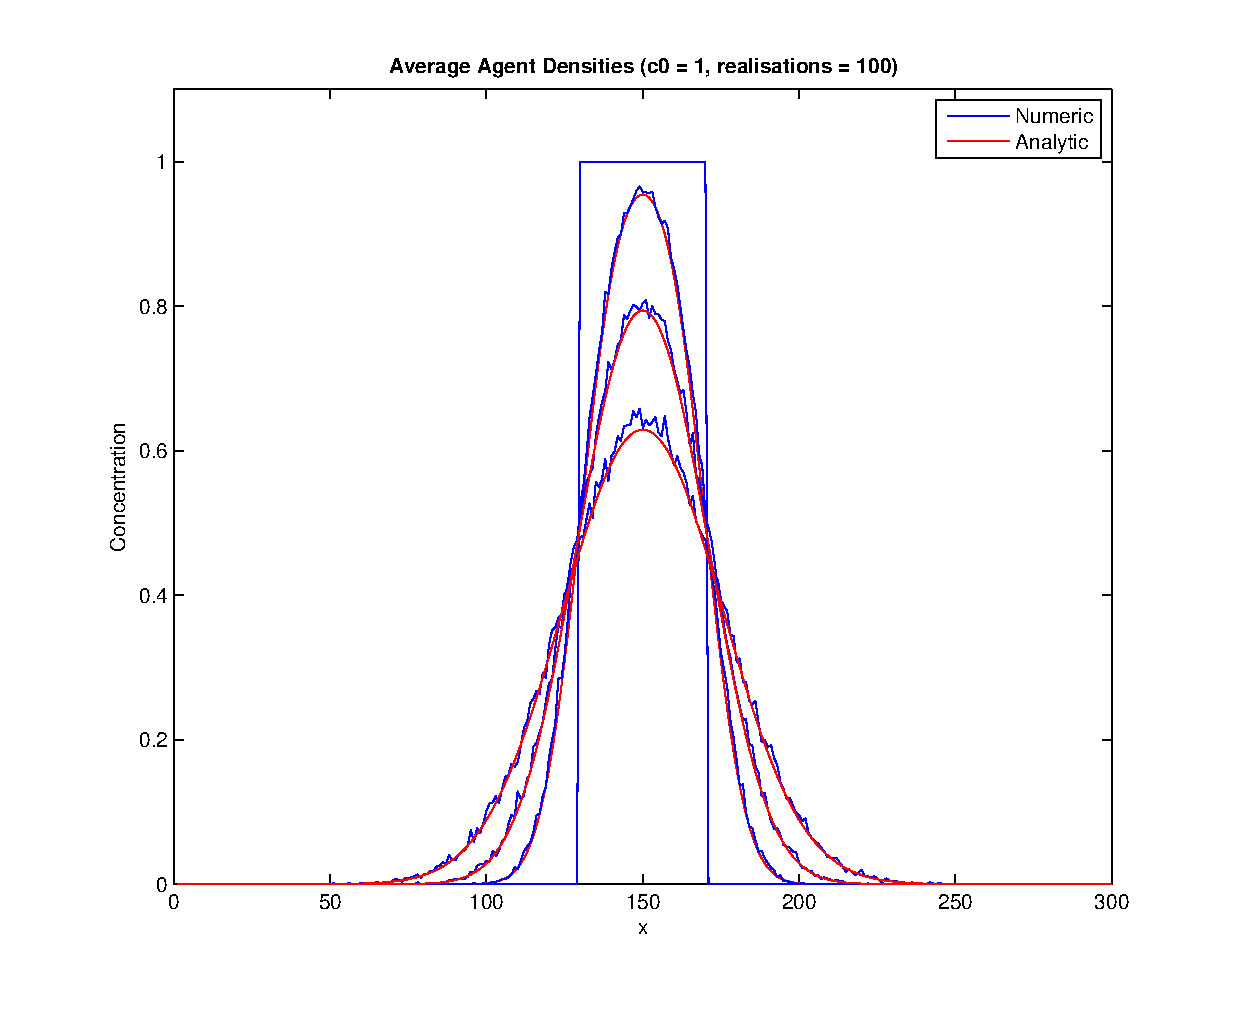
\includegraphics[width=\textwidth]{./Figures/cell_concentration_1_100.eps}
			\caption{Comparison of agent density between a random walk model and the diffusion equation. The model had volume exclusion with unbiased motility and no proliferation. Density data was obtained by averaging the occupancy of each column over 100 identically-prepared realisations satisfying (\ref{eq:ivp_ic}) where $C_0 = 1$. Densities are given at $t = 0, 200, 500,$ and $1000$ and shows agent density diffusing across the lattice.}
			\label{fig:cell_concentration_1_100}
		\end{figure}
	
		Additional simulations were conducted in thoroughly examining the random walk model. As expected from (\ref{eq:analytic_con_prolif}), modifying $C_0$ merely scales the agent density curves (see Figure \ref{fig:cell_concentration_5_100}). Furthermore, as expected by the Law of Large Numbers, the accuracy of the reproduced model was dependent on the number of realisations averaged over \cite{lawlargenum}. As seen between Figures \ref{fig:cell_concentration_1_100} and \ref{fig:cell_concentration_1_10}, an increase in the total realisations performed results in higher accuracy in the final solution.
	
		\begin{figure}[tbh]
			\centering
				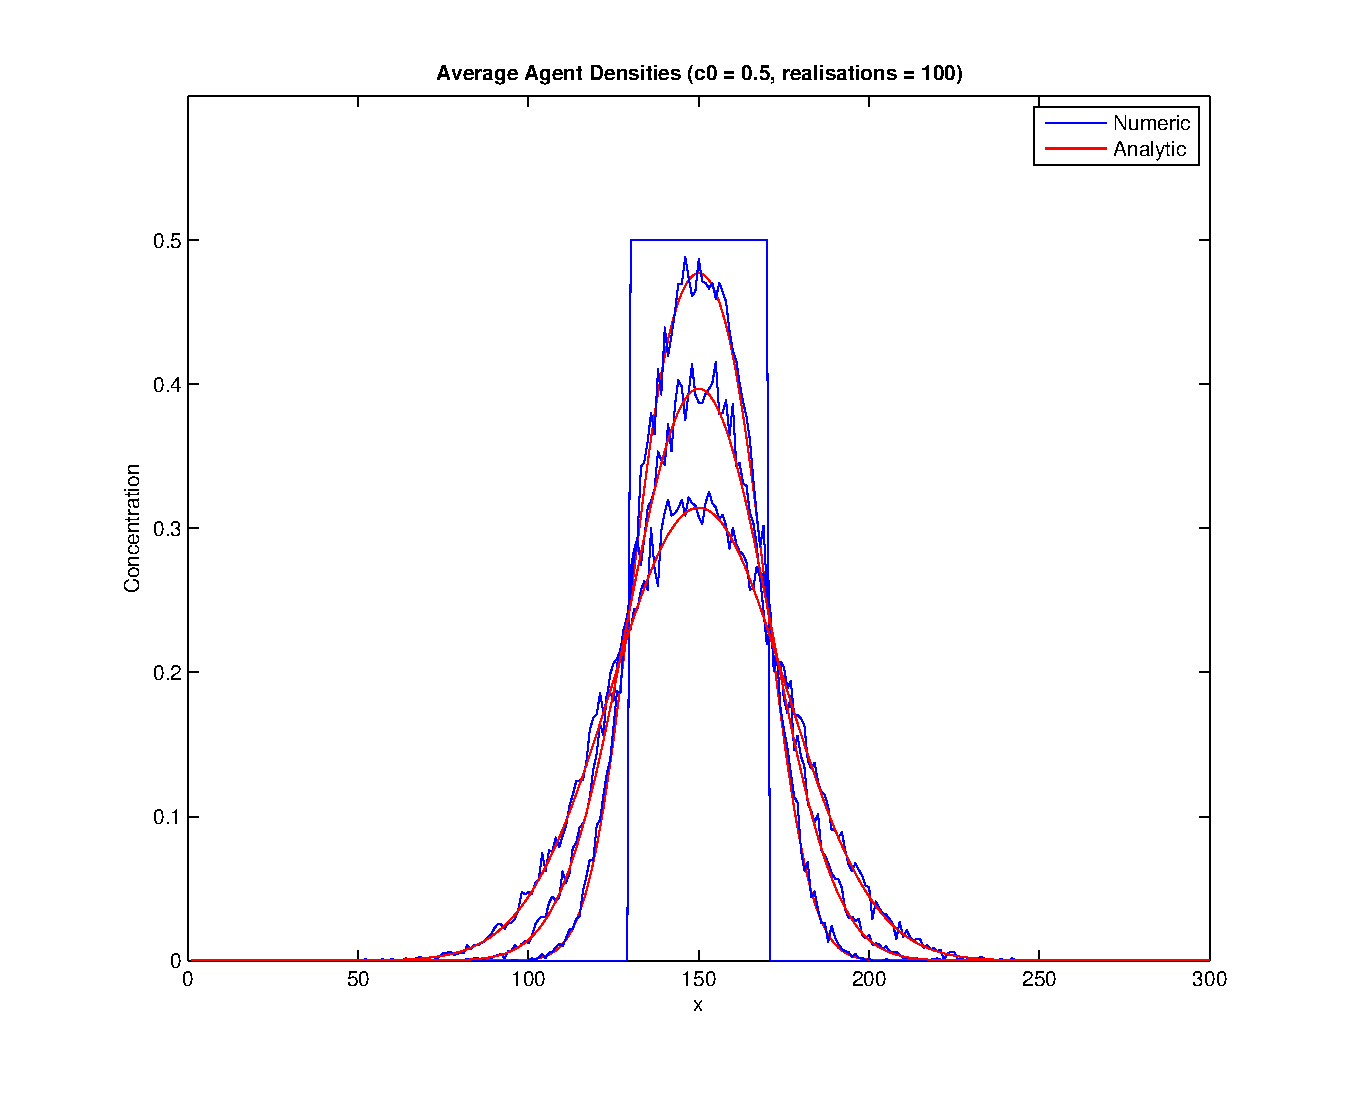
\includegraphics[width=\textwidth]{./Figures/cell_concentration_5_100.eps}
			\caption{Comparison of agent density between a random walk model and the diffusion equation. The model had volume exclusion with unbiased motility and no proliferation. Density data was obtained by averaging the occupancy of each column over 100 identically-prepared realisations satisfying (\ref{eq:ivp_ic}) where $C_0 = 0.5$. Densities are given at $t = 0, 200, 500,$ and $1000$ and shows agent density diffusing across the lattice.}
			\label{fig:cell_concentration_5_100}
		\end{figure}

		\begin{figure}[tbh]
			\centering
				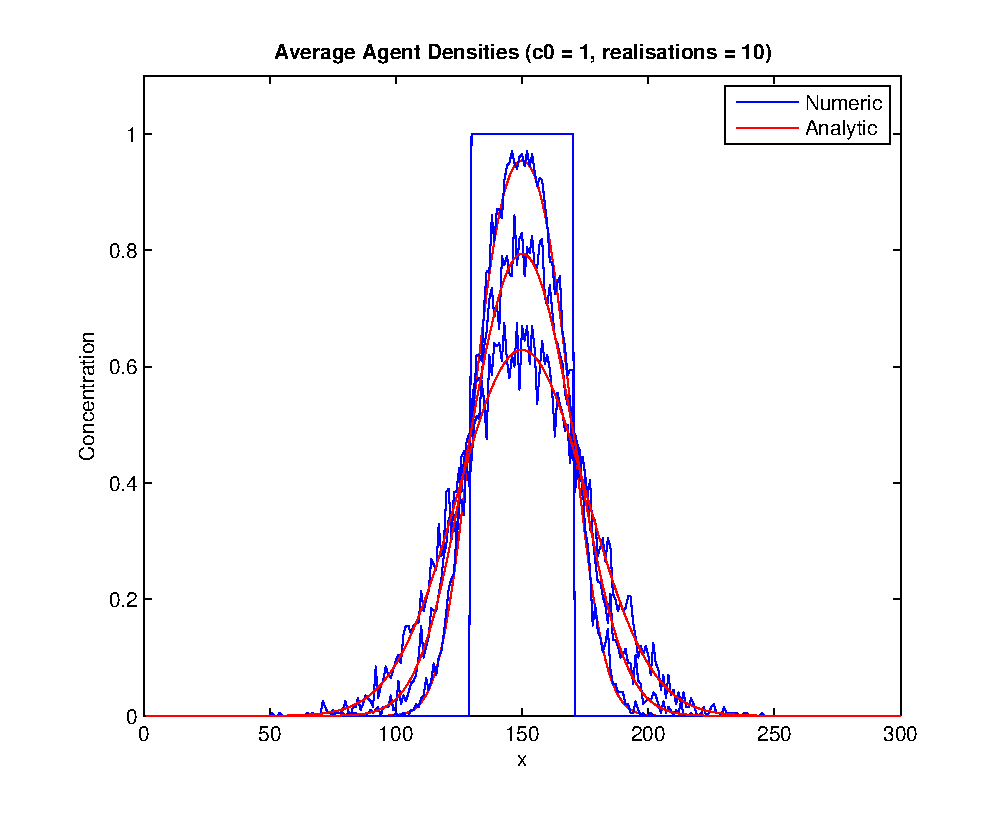
\includegraphics[width=\textwidth]{./Figures/cell_concentration_1_10.eps}
			\caption{Comparison of agent density between a random walk model and the diffusion equation. The model had volume exclusion with unbiased motility and no proliferation. Density data was obtained by averaging the occupancy of each column over 10 identically-prepared realisations satisfying (\ref{eq:ivp_ic}) where $C_0 = 1$. Densities are given at $t = 0, 200, 500,$ and $1000$ and shows agent density diffusing across the lattice.}
			\label{fig:cell_concentration_1_10}
		\end{figure}
	
	% end sub:results

% end sec:simrandin2d

\section{Random Lattices in 1D}
	\label{sec:randlatticein1d}
	
	In simulating cellular phenomena via random walk models, there exists three common methods for handling the spatial domain of interest: equally-spaced lattices, random lattices, and lattice free models. Lattices can be used under a variety of circumstances to discretise the spatial domain into a distinct set of nodes, which cells can consequently occupy. As discussed by Simpson \cite{simpson2010cell}, lattices can be constructed based off the expected size of a cell and the approximate distance they may move over a period of time. In constructing an equally-spaced lattice, nodes are spaced uniformly throughout a domain. Alternatively, nodes are positioned randomly or pseudorandomly within a domain in constructing a random lattice. Unfortunately, cells do not exhibit movement in a rigid, discrete manner, hence lattice-based models may not accurately simulate certain biological processes \cite{plank2013lattice}. Lattice free models avoid this issue by not imposing a spatial discretisation on the simulations, which results in a major performance penalty. 

	Research was conducted into the application of random lattices in simulating cell motility in one dimension. Two approaches were taken in constructing a random lattice: perturbing an equally-spaced lattice and generating node locations pseudorandomly. Let $x_i$ be the position of the $i^\text{th}$ node in the lattice. Under the perturbing approach, each node position is given by:
	\begin{equation*}
		x_i = y_i + \Phi
	\end{equation*}
	where $y_i$ is the location of the $i^{\text{th}}$ unpertubed node in the equally-spaced lattice and $\Phi$ is a random variable. Under the pseudorandom approach, each node position is given by:
	\begin{equation*}
		x_i = \Theta
	\end{equation*}
	where $\Theta$ is a random variable. For all simulations, pseudorandom numbers were sourced from a variety of distributions using Intel's Vector Statistical Library (VSL).

	\subsection{The Perturbing Approach}
		\label{sub:theperturbingapproach}
		
		\subsubsection{Lattice Properties}
		\label{sub:latticeproperties_perturbed}
			
			Initially, several key characteristics of lattices were identified in determining the preferred method for generating random lattices. The deltas between adjacent nodes and the existence of node clusters were of particular interest in generating physically realistic lattices for simulating cellular phenomenon. A series of random lattices were constructed on a dimensionless 1D region of 20 dimensionless length units in which 20 nodes would be positioned. For the perturbation method, the equally-spaced lattice consisted of 20 nodes spaced one length unit apart with the first node residing at position zero. 

			Figure \ref{fig:perturbed_layout_1} depicts random lattices generated using the perturbation approach given by the continuous random variable
			\begin{equation}
				\label{eq:perturb_dist}
				\Phi \sim \text{Uniform}(-\delta x, \delta x)
			\end{equation}
			where $\delta x$ is the maximum absolute perturbation allowed. These results quickly revealed that large perturbations are detrimental to the construction of random lattices since node clustering is evident. For example, consider the lattices where $\delta x = 0.1$ and $\delta x = 0.5$. The former closely resembles an equally-spaced lattice whereas the latter exhibits node clustering around $x = 6$ and $x = 13$ and large unoccupied regions around $x = 5$. Such disparity in lattice spacing can result in erroneous simulations since cell motility can be subject to large variations in the distance travelled per unit time. These findings are exacerbated as $\delta x$ is increased further, which can be shown by considering the expected value and variance of the deltas between adjacent nodes.

			\begin{figure}[tbh]
				\centering
					\includegraphics[width=\textwidth]{/Figures/perturbed_layout_1.eps}
				\caption{A series of randomly populated lattices generated by perturbing an equally-spaced lattice. Perturbations are sourced from a uniform distribution whose range is defined by a maximum allowable perturbation delta $\delta x$ as given by (\ref{eq:perturb_dist}). The investigated $\delta x$ values range from $0.1$ to $0.5$.}
				\label{fig:perturbed_layout_1}
			\end{figure}

			Consider a random lattice generated using the perturbing approach and given the unperturbed lattice has a fixed node spacing $\Delta x$. Let $A$ and $B$ be independent, identically distributed random variables. The expected node spacing is given by:
			\begin{align*}
				\mathrm{E} \left(x_i - x_{i-1} \right) &= \mathrm{E} \left(y_i + A - y_{i-1} - B \right) \\
				&= \mathrm{E} \left(\Delta x + A - B \right) \\
				&= \Delta x + \mathrm{E} \left(A \right) - \mathrm{E} \left(B \right) \\
				&= \Delta x.
			\end{align*}
			As such, if we were to investigate the average delta between adjacent nodes over numerous meshes, then by the Law of Large Numbers the expected delta is that of the equally-spaced lattice. This finding does not explicitly describe the existence of node clustering and large deltas between nodes as seen previously. Instead, consider finding the variance of the same statistic as follows:
			\begin{align*}
				\mathrm{Var} \left(x_i - x_{i-1} \right) &= \mathrm{Var} \left(y_i + A - y_{i-1} - B \right) \\
				&= \mathrm{Var} \left(\Delta x + A - B \right) \\
				&= \mathrm{Var} \left(A - B \right) \\
				&= \mathrm{Var} \left(A \right) + \mathrm{Var} \left(B \right) - 2 \mathrm{Cov} \left(A, B \right) \\ 
				&= \mathrm{Var} \left(A \right) + \mathrm{Var} \left(B \right) - 2 \mathrm{E} \left(AB \right) + 2 \mathrm{E} \left(A \right) \mathrm{E} \left(B \right) \\ 
				&= 2 \mathrm{Var} \left(A \right)
			\end{align*}
			noting that $\mathrm{Var} \left(A \right) = \mathrm{Var} \left(B \right)$. Therefore the variability in the deltas between adjacent nodes is linearly proportional to the variance of the distribution from which perturbations are sourced from.
		
			These same results were exhibited by averaging adjacent node spacings over a series of random lattices. For differing values of $\delta x$, 100 random lattices were generated in which 40 nodes were placed over a 1D region consisting of 40 dimensionless length units. As seen in Figure \ref{fig:perturbed_node_spacings_boxplots_lattices}, the variability in minimum and maximum node spacings tends to increase linearly with $\delta x$. Furthermore, the mean node spacing (not shown) consistently converges to the expected value of $\Delta x = 1$ by the Law of Large Numbers. Additional analysis was conducted into the identification of node clustering in the absence of averaging, however, the results were somewhat inconclusive due to randomness and are not discussed here. 

			\begin{figure}[tbh]
				\centering
					\includegraphics[width=\textwidth]{/Figures/perturbed_node_spacings_boxplots_lattices.eps}
				\caption{Boxplots of the spacing between adjacent nodes as collected over 100 random lattices for varying values of $\delta x$. Each random lattice consisted of 40 nodes spread over 40 dimensionless length units. The investigated $\delta x$ values range from $0.1$ to $0.5$.}
				\label{fig:perturbed_node_spacings_boxplots_lattices}
			\end{figure}

		% end subs:latticeproperties_perturbed

		\subsubsection{Simulating Random Walks}
		\label{sub:simulatingrandomwalks_perturbed}
			
			Random walks were conducted on perturbed lattices to obtain information regarding how such perturbations may impact cell motility. As per Simpson's analysis \cite{simpson2009diffusing}, the net agent displacement,
			\begin{equation}
				\label{eq:netDisplacement}
				X_t - X_0 = \sum_{i = 1}^{t} \left (X_i - X_{i-1} \right),
			\end{equation}
			and the sum of squared displacements,
			\begin{equation}
				\label{eq:sumSquaredDisplacement}
				S_t = \sum_{i = 1}^{t} \left (X_i - X_{i-1} \right)^2,
			\end{equation}
			were investigated for different reasons. Note carefully the distinction between $X_i$ and $x_i$: $X_i$ is the location of a cell at the $i^\text{th}$ time step whereas $x_i$ is the location of the $i^\text{th}$ node. The net displacement gives information on how a cell displaces itself from its starting position. Given the random walk method described section \ref{sec:simrandin2d}, it is expected that the net displacement should fluctuate about zero. On the other hand, the sum of square displacements is used to describe how the cell moves over the course of the simulation. As such, fluctuations can be observed as a cell travels over large distances and within node clusters, which is not adequately represented by (\ref{eq:netDisplacement}). The expected sum of squared displacements is
			\begin{equation}
				\label{eq:expectedSumSquaredDisp}
				\mathrm{E} \left(S_t \right) = \sum_{i = 1}^{t} \mathrm{E} \left( \left(X_i - X_{i-1} \right)^2 \right)
			\end{equation}
			by the linearity of the expected value operator. Let $A$, $B$, and $C$ be independent, identically distributed random variables and $\Delta x$ be the spacing between nodes on the equally-spaced lattice. Additionally, suppose that at the $i^\text{th}$ time step the cell is located at $x_j$. Now consider
			\begin{align*}
				\mathrm{E} \left( \left(X_i - X_{i-1} \right)^2 \right) &= \mathrm{E} \left( \frac{1}{2} \left(x_{j+1} - x_j \right)^2 + \frac{1}{2} \left(x_{j-1} - x_j \right)^2 \right) \\
				&= \frac{1}{2} \mathrm{E} \left(\left(x_{j+1} - x_j \right)^2 \right) + \frac{1}{2} \mathrm{E} \left(\left(x_{j-1} - x_j \right)^2 \right) \\
				&= \frac{1}{2} \mathrm{E} \left(\left(\Delta x + A - B \right)^2 \right) + \frac{1}{2} \mathrm{E} \left(\left(\Delta x + C - B \right)^2 \right).
			\end{align*}
			For brevity, consider
			\begin{align*}
			\frac{1}{2} \mathrm{E} \left(\left(\Delta x + A - B \right)^2 \right) &= \frac{1}{2} {\Delta x}^2 + \Delta x \mathrm{E} \left (A - B \right) + \frac{1}{2} \mathrm {E} \left( \left(A - B \right)^2 \right) \\
			&= \frac{1}{2} {\Delta x}^2 + \frac{1}{2} \left(\mathrm{E} \left(A^2 \right) - 2 \mathrm{E} \left(AB \right) + \mathrm{E} \left(B^2 \right) \right).
			\end{align*}
			Noting that $A$, $B$, and $C$ and independent and $\mathrm{Var} \left(A \right) = \mathrm{Var} \left(B \right) = \mathrm{Var} \left(C \right)$,
			\begin{align*}
			\frac{1}{2} \mathrm{E} \left(\left(\Delta x + A - B \right)^2 \right) &= \frac{1}{2} {\Delta x}^2 + \frac{1}{2} \left(\mathrm{E} \left(A^2 \right) - \mathrm{E} \left(A \right)^2 + \mathrm{E} \left(B^2 \right) - \mathrm{E} \left(B \right)^2 \right) \\
			&= \frac{1}{2} {\Delta x}^2 + \frac{1}{2} \left(\mathrm{Var} \left(A \right) + \mathrm{Var} \left(B \right) \right) \\
			&= \frac{1}{2} {\Delta x}^2 + \mathrm{Var} \left(B \right).
			\end{align*}
			Applying this result in simplifying (\ref{eq:expectedSumSquaredDisp}), gives
			\begin{align*}
				\mathrm{E} \left( \left(X_i - X_{i-1} \right)^2 \right) &= \frac{1}{2} {\Delta x}^2 + \mathrm{Var} \left(B \right) + \frac{1}{2} {\Delta x}^2 + \mathrm{Var} \left(B \right) \\
				&= {\Delta x}^2 + 2 \mathrm{Var} \left(B \right),
			\end{align*}
			therefore,
			\begin{equation}
				\label{eq:expectedSumSquaredDispAns}
				\mathrm{E} \left(S_t \right) = t \left({\Delta x}^2 + 2 \mathrm{Var} \left(B \right) \right).
			\end{equation}
			Using a similar approach as above, in the absence of perturbation it can be shown that, 
			\begin{equation}
				\label{eq:expectedSumSquaredDispNoPerturbAns}
				\mathrm{E} \left(S_t \right) = t {\Delta x}^2.
			\end{equation}
			Alternatively, consider the case where there is no variance in the perturbations, which is equivalent to translating the domain of interest. In this case, (\ref{eq:expectedSumSquaredDispAns}) clearly reduces to (\ref{eq:expectedSumSquaredDispNoPerturbAns}). Therefore, as the variance in perturbations increases so does $\mathrm{E} \left(S_t \right)$.

			Random walk simulations of a single agent (i.e. cell) were conducted over a series of lattices in ensuring the averaged results matched (\ref{eq:expectedSumSquaredDispAns}) and (\ref{eq:expectedSumSquaredDispNoPerturbAns}). Initially, equally-spaced lattices were considered for 500 time steps. Periodic boundary conditions were applied but never encountered by the agent by making the ratio of $\Delta x$ and the length of the domain sufficiently small given the number of time steps. Linear least-squares fits were made to both the net displacement and the sum of squared displacements in comparing the results to the expected solutions. As seen in Figure \ref{fig:disp_equidistance_1_lattice}, given that $\Delta x = 1$, the results match the expected solutions well with a fitted gradient for $S_t$ of approximately $1.0$. 

			\begin{figure}[tbh]
				\centering
					\includegraphics[width=\textwidth]{/Figures/disp_equidistance_1_lattice.eps}
				\caption{The progression of $S_t$ and $X_t - X_0$ for a single agent over time on an equally-spaced lattice with $\Delta x = 1$. Linear least-squares fits were made from this data where the resultant functions were constrained to pass through $(0,0)$. The fitted gradient for $S_t$ was $1.0$ and for $X_t - X_0$ it was $0.0$ (rounded to one decimal place).}
				\label{fig:disp_equidistance_1_lattice}
			\end{figure}

			As increasily large perturbations are introduced, the value of $\mathrm{E} \left(S_t \right)$ increased. For example, individual walks were conducted on 100 perturbed lattices where perturbations were sourced from (\ref{eq:perturb_dist}) for $\delta x = 0.5$ and $\Delta x = 1$. As seen in Figure \ref{fig:disp_perturbed_50_100_lattices}, the expected value of $S_t$ has increased with $\delta x$ compared to Figure \ref{fig:disp_equidistance_1_lattice}. Under such a perturbation scheme, the expected gradient of $S_t$ is  
			\begin{equation*}
				\text{m} = {\Delta x}^2 + 2 \mathrm{Var} \left(B \right) =  1 + \frac{1}{6} = \frac{7}{6} = 1.1\overline{6}.
			\end{equation*}
			The fitted gradients of $1.16$ for $S_t$ and $0.0$ for $X_t - X_0$ match the expected values quite well. The expected result was reproduced for a variety of values for $\delta x$.

			\begin{figure}[tbh]
				\centering
					\includegraphics[width=\textwidth]{/Figures/disp_perturbed_50_100_lattices.eps}
				\caption{The progression of $S_t$ and $X_t - X_0$ for a single agent over time averaged over 1000 perturbed lattices with $\Delta x = 1$ and perturbations sourced from (\ref{eq:perturb_dist}). Linear least-squares fits were made from this data where the resultant functions were constrained to pass through $(0,0)$. The fitted gradient for $S_t$ was $1.16$ and for $X_t - X_0$ it was $0.0$ (rounded to two decimal places).}
				\label{fig:disp_perturbed_50_100_lattices}
			\end{figure}

			The expected solutions derived earlier are general enough to apply to a variety of distributions. For example, perturbations were sourced from a Gaussian distribution with a mean of zero and a standard deviation of $0.2887$. This standard deviation provides a variance equivalent to that of (\ref{eq:perturb_dist}) with $\delta x = 0.5$, whose results are seen in Figure \ref{fig:disp_perturbed_50_100_lattices}. Unsurprisingly, the same results are generated by sourcing from the aforementioned Gaussian distribution (Figure \ref{fig:displacements_perturbed_single_lattices_g_29_high}).

			\begin{figure}[tbh]
				\centering
					\includegraphics[width=\textwidth]{/Figures/displacements_perturbed_single_lattices_g_29_high.eps}
				\caption{The progression of $S_t$ and $X_t - X_0$ for a single agent over time averaged over 1000 perturbed lattices with $\Delta x = 1$ and perturbations sourced from a Gaussian distribution with mean zero and a standard deviation of $0.2887$. Linear least-squares fits were made from this data where the resultant functions were constrained to pass through $(0,0)$. The fitted gradient for $S_t$ was $1.16$ and for $X_t - X_0$ it was $0.0$ (rounded to two decimal places).}
				\label{fig:displacements_perturbed_single_lattices_g_29_high}
			\end{figure}

		% end subs:simulatingrandomwalks_perturbed 
	
		\subsubsection{Pertubing and Diffusivity}
			\label{subs:pertubinganddiffusivity}
			
			As outlined in section \ref{sub:results}, Simpson showed the diffusion equation can be used to describe certain cellular processes when simulated on an equally-spaced lattice. It was consequently investigated whether such an analytic solution also applies to simulations conducted on a perturbed lattice. 

			Initially, simulations were designed and conducted to compare (\ref{eq:analytic_con_prolif}) with (\ref{eq:ivp_ic})) (i.e. the diffusion equation) against agent density data averaged over multiple realisations. A series of simulations were performed for a one-dimensional equivalent of the model detailed in section \ref{sub:results}. Instead of visualising the random walks on an equally-spaced lattice, however, a perturbed lattice was used instead. As seen in Figure \ref{fig:densities_2000_1}, the averaged simulation data fits the diffusion equation quite well. Similar results were obtained for $\delta x < \sfrac{\Delta x}{2}$.
		
			\begin{figure}[tbh]
				\centering
					\includegraphics[width=\textwidth]{/Figures/densities_2000_1.eps}
				\caption{Comparison of agent density between a random walk model and the diffusion equation. The model had volume exclusion with unbiased motility and no proliferation. The random walks were visualised on a random lattice generated using the perturbation approach with $\delta x = 0.1$. Density data was obtained by averaging the occupancy of each column over 2000 identically-prepared realisations satisfying (\ref{eq:ivp_ic}) where $C_0 = 1$. Densities are given at $t = 0, 200, 500,$ and $1000$ and shows agent density diffusing across the lattice.}
				\label{fig:densities_2000_1}
			\end{figure}

			Originally, Simpson considered a one-dimensional agent conservation statement in showing that the diffusion equation can be used to describe certain cellular phenomenon. Let $C_i(t)$ denote averaged agent occupancy (i.e. concentration) at the $i^{\text{th}}$ node at time $t$. Consider a random walk model with volume exclusion and unbiased cell motility. If an agent is chosen for action, suppose that there is probability $P$ that the agent attempts to move. As such, the conservation of agent statement at $x_i$ is:
			\begin{equation}
			  	\phantom{C(x_i, t + \delta t) - C(x_i, t)}
			  	\begin{aligned}
			    	\mathllap{C_i(t + \delta t) - C_i(t)} &= C_{i-1}(t) \frac{P}{2} \left(1 - C_i(t) \right) + C_{i+1}(t) \frac{P}{2} \left(1 - C_i(t) \right)\\
			      	&\qquad  - C_i(t) \frac{P}{2} \left(1 - C_{i-1}(t) \right) - C_i(t) \frac{P}{2} \left(1 - C_{i+1}(t) \right)
			  	\end{aligned}
			  	\label{eq:conservationst}
		  	\end{equation}
			where $\delta t$ is the time step size. This statement is a simplification of Simpson's agent conservation statement in two-dimensions with support for biased motility \cite{simpson2009diffusing}. Note carefully that due to volume exclusion $0 \le C_i(t) \le 1$, hence agent motility events can only occur if the designated move location is vacant. Expanding (\ref{eq:conservationst}) gives
			\begin{align*}
			  	\phantom{C(x_i, t + \delta t) - C(x_i, t)}
			  	&\begin{aligned}
			    	\mathllap{C_i(t + \delta t) - C_i(t)} &= \frac{P}{2} \left(C_{i-1}(t) - C_{i-1}(t)C_i(t) \right) + \frac{P}{2} \left(C_{i+1}(t) - C_{i+1}(t)C_i(t) \right) \\
			      	&\qquad - \frac{P}{2} \left(C_i(t) - C_i(t)C_{i-1}(t) \right) - \frac{P}{2} \left(C_i(t) - C_i(t)C_{i+1}(t) \right)
			  	\end{aligned}\\
			  	&\begin{aligned}
			    	\mathllap{} &= \frac{P}{2} \left(C_{i-1}(t) - 2 C_i(t) + C_{i+1}(t) \right).
			  	\end{aligned}
		  	\end{align*}
		  	Dividing by $\delta t$ gives the standard finite difference approximation on the right-hand side:
		  	\begin{align}
			  	\phantom{\frac{C(x_i, t + \delta t) - C(x_i, t)}{\delta t}}
			  	&\begin{aligned}
			    	\mathllap{\frac{C_i(t + \delta t) - C_i(t)}{\delta t}} &= \frac{P}{2 \delta t} \left(C_{i-1}(t) - 2 C_i(t) + C_{i+1}(t) \right).
			    \end{aligned}
			    \label{eq:conservationSimplified}
		  	\end{align}
		  	Let $\alpha_i$ be the difference between node $i$ and $i-1$ as determined by the perturbation approach. Therefore,
		  	\begin{equation*}
		  		\alpha_i = \Delta x - A_i + B_i
		  	\end{equation*}
		  	where $A_i$ and $B_i$ independent, identically distributed random variables with an expected value of zero as defined by (\ref{eq:perturb_dist}). Alternatively,
		  	\begin{equation*}
		  		\alpha_i = \Delta x + r_i
		  	\end{equation*}
		  	where $r_i$ is a random variable given by $r_i = B_i - A_i$. Let $x_i$ be the position of $i^{\text{th}}$ node, now $C_{i-1}(t)$ (i.e. $C(x_{i-1}, t)$) and $C_{i+1}(t)$ (i.e. $C(x_{i+1}, t)$) can be approximated by a second Taylor series centred at $x_i$ as follows: 
		  	\begin{align*}
			  	\phantom{C(x_{i-1}, t)}
			  	&\begin{aligned}
			    	\mathllap{C(x_{i-1}, t)} &=  C_i(t) - \frac{\partial C}{\partial x}\bigg|_{x=x_i} \left (\Delta x + r_{i-1} \right) + \frac{1}{2} \frac{\partial^2 C}{\partial x^2}\bigg|_{x=x_i} \left (\Delta x + r_{i-1} \right)^2 \\
			    	&\qquad - \text{O} \left( \left(\Delta x + r_{i-1} \right)^3 \right)
			    \end{aligned}
		  	\end{align*}
		  	\begin{align*}
		  		\phantom{C(x_{i+1}, t)}
		  		&\begin{aligned}
			    	\mathllap{C(x_{i+1}, t)} &=  C_i(t) + \frac{\partial C}{\partial x}\bigg|_{x=x_i} \left (\Delta x + r_{i+1} \right) + \frac{1}{2} \frac{\partial^2 C}{\partial x^2}\bigg|_{x=x_i} \left (\Delta x + r_{i+1} \right)^2 \\
			    	&\qquad + \text{O} \left( \left(\Delta x + r_{i+1} \right)^3 \right).
			    \end{aligned}
		  	\end{align*}
		  	Substituting these equations into (\ref{eq:conservationSimplified}) gives, 
		  	\begin{align*}
			  	\phantom{\frac{C(x_i, t + \delta t) - C(x_i, t)}{\delta t} \frac{2 \delta t}{P}}
			  	&\begin{aligned}
			    	\mathllap{\frac{C_i(t + \delta t) - C_i(t)}{\delta t} \frac{2 \delta t}{P}} &=  \left(\Delta x + r_{i+1} \right) \frac{\partial C}{\partial x}\bigg|_{x=x_i} - \left(\Delta x + r_{i-1} \right) \frac{\partial C}{\partial x}\bigg|_{x=x_i} \\
			    	&\qquad + \frac{1}{2} \frac{\partial^2 C}{\partial x^2}\bigg|_{x=x_i} \left (\Delta x + r_{i+1} \right)^2 \\
			    	&\qquad + \frac{1}{2} \frac{\partial^2 C}{\partial x^2}\bigg|_{x=x_i} \left (\Delta x + r_{i-1} \right)^2 \\
			    	&\qquad + \BigO{\left(\Delta x + r_{i+1} \right)^3} + \BigO{\left(\Delta x + r_{i-1} \right)^3}
			    \end{aligned}
		  	\end{align*}
		  	Given $r_i \ll \Delta x$,
		  	\begin{align*}
			  	\phantom{\frac{C(x_i, t + \delta t) - C(x_i, t)}{\delta t} \frac{2 \delta t}{P}}
			  	&\begin{aligned}
			    	\mathllap{\frac{C_i(t + \delta t) - C_i(t)}{\delta t} \frac{2 \delta t}{P}} &= {\Delta x}^2 \frac{\partial^2 C}{\partial x^2}\bigg|_{x=x_i} + \BigO{2 {\Delta x}^3} + \BigO{\text{Max} \left({r_i}^2 \right)}.
			    \end{aligned}
		  	\end{align*}
		  	Now, taking the limit as $\Delta x \to 0$ and $\delta t \to 0$ whilst keeping $\sfrac{{\Delta x}^2}{\delta t}$ constant \cite{codling2008random}, the error terms are removed and the discrete derivative in time is replaced by it's continuous analogue giving
		  	\begin{equation*}
		  		\frac{\partial C}{\partial t} = D \frac{\partial^2 C}{\partial x^2}
		  	\end{equation*}
		  	where 
		  	\begin{equation*}
		  		D = \lim_{\Delta x, \delta t \to 0} \left( \frac{P {\Delta x}^2}{2 \delta t}\right).
		  	\end{equation*}
		  	This governing PDE is equivalent to that derived by Simpson for equally-spaced lattices \cite{simpson2009diffusing}. This finding shows that a random lattice does not influence simulation results provided the perturbations are sufficiently small compared to $\Delta x$. This is interesting considering that the diffusivity of a single cell is influenced by the distribution perturbations are sourced from. Any influence on the diffusivity of a single cell could be negated in the presence of volume exclusion, which was not considered in the derivation of (\ref{eq:expectedSumSquaredDispAns}). Further investigation into this finding was planned for future work.

		% end subs:pertubinganddiffusivity

	% end sub:theperturbingapproach

	\subsection{The Random Approach}
		\label{sub:therandomapproach}
		
		\subsubsection{Lattice Properties}
			\label{subs:latticeproperties_random}
			
			Equivalent simulations were conducted for the random and perturbing approaches to facilitate comparison. As such, a series of random lattices were constructed on a dimensionless 1D region of 20 dimensionless length units consisting of 20 nodes. Figure \ref{fig:pseudo_layout_1} depicts a series of random lattices generated by the random approach where
			\begin{equation}
				\label{eq:random_dist}
				\Theta \sim \text{Uniform} \left(0, 20\right).	
			\end{equation}
			In comparison to Figure \ref{fig:pseudo_layout_1}, the random approach exhibits node clustering quite clearly. This is expected given that the random approach is greatly influenced by stochastic processes compared to the perturbed approach where $\Delta x \gg \text{Max} \left(\Phi \right)$. Therefore, any node clustering and large deltas between adjacent nodes can be avoided by sourcing a large number of node positions in creating a fine lattice.

			\begin{figure}[tbh]
				\centering
					\includegraphics[width=\textwidth]{/Figures/pseudo_layout_1.eps}
				\caption{A series of randomly populated lattices generated by sourcing node positions from a uniform distribution spanning the region of interest as given by (\ref{eq:random_dist}). Multiple lattices are displayed to illustrate the variability between lattices generated using this approach.}
				\label{fig:pseudo_layout_1}
			\end{figure}

		% end subs:latticeproperties_random

		\subsubsection{Simulating Random Walks}
		\label{sub:simulatingrandomwalks_random}
			
			Using approaches similar to those applied in section \ref{sub:simulatingrandomwalks_perturbed}, it can be shown that
			\begin{equation*}
				\mathrm{E} \left(X_t - X_0 \right) = 0
			\end{equation*}
			and 
			\begin{equation*}
				\mathrm{E} \left(S_t \right) = 2 t \mathrm{Var} \left(\Theta \right)
			\end{equation*}
			where $\Theta$ is the random variable defining the locations the nodes. Several sets of simulations were designed and executed in an attempt to reproduce the expected results. Due to the large impact that stochastic processes have on this method it was computationally infeasible to construct simulations which would be impacted by the Law of Large Numbers. Meshes would need to be extremely fine or a large number of simulations would need to be run to compensate for the variability. As such, generating random meshes using a purely pseudorandom method is arguably unsuitable for large scale simulations or applications which do not require a fine mesh. 
		
		% end subs:simulatingrandomwalks_random 
	
	% end sub:thepurelypseudorandomapproach

% end sec:randlatticein1d

\section{Investigating Travelling Wave Solutions}
	\label{sec:investigatingfishersequation}
	
	\subsection{Phase Plane Analysis of Fisher's Equation}
		\label{sub:phaseplaneanalysisoffishersequation}
		
		As stated in section \ref{sub:results}, several PDEs were derived in Simpson's prior work in describing cellular phenomenon. For certain biological processes, variants of Fisher's equation can be used as a governing equation \cite{simpson2009diffusing}. As such, the travelling wave solutions of Fisher's equation for population growth,
		\begin{equation}
			 \label{eq:fisherseq}
			 \frac{\partial U}{\partial t} = \nu \frac{\partial^2 U}{\partial y^2} + k U (1 - U),
		\end{equation}
		was thoroughly analysed via \cite{canosa1973nonlinear}. To ease subsequent analysis, (\ref{eq:fisherseq}) can be nondimensionalised via the unit-reducing substitutions:
		\begin{align}
			 \label{eq:timeSubFisher}
			 \tau &= \alpha t \qquad \text{and} \\
			 \label{eq:spaceSubFisher} 
			 x &= \beta y
		\end{align}
		where $\alpha$ and $\beta$ have units $t^{-1}$ and $m^{-1}$, respectively. Applying the substitution in (\ref{eq:timeSubFisher}) and the chain rule, we obtain:
		\begin{align*}
			 \frac{\partial U}{\partial \tau} \frac{d \tau}{d t} &= \nu \frac{\partial^2 U}{\partial y^2} + k U (1 - U) \\ 
			 \alpha \frac{\partial U}{\partial \tau} &= \nu \frac{\partial^2 U}{\partial y^2} + k U (1 - U)
		\end{align*}
		By inspection, it is clear that (\ref{eq:fisherseq}) can be nondimensionalised in time and simplified when $\alpha = k$. Hence,
		\begin{equation}
			 \label{eq:timeSubbedFisher}
			 \frac{\partial U}{\partial \tau} = \frac{\nu}{k} \frac{\partial^2 U}{\partial y^2} + U (1 - U)
		\end{equation}
		Applying (\ref{eq:spaceSubFisher}) in a similar manner gives
		\begin{equation*}
			 \frac{\partial U}{\partial \tau} = \frac{\beta^2 \nu}{k} \frac{\partial^2 U}{\partial x^2} + U (1 - U).
		\end{equation*}
		As such, (\ref{eq:timeSubbedFisher}) can be nondimensionalised in space and simplified when $\beta = \sqrt{\sfrac{k}{\nu}}$, which results in
		\begin{equation}
			 \label{eq:timeSpaceSubbedFisher}
			 \frac{\partial U}{\partial \tau} = \frac{\partial^2 U}{\partial x^2} + U (1 - U).
		\end{equation}
		As discussed by Canosa \cite{canosa1973nonlinear}, this nondimensionalised equation describes nonlinear population growth in one spatial dimension. Consequently, the modelled habitat (i.e. space) can only feasibly support a maximum population per unit length. Given the form of the logistic source term in (\ref{eq:timeSpaceSubbedFisher}), the maximum population is unity. The following initial condition can therefore be applied:
		\begin{equation}
			 \label{eq:fisherInitialCondition}
			 0 \le U(x, 0) \le 1, \qquad -\infty < x < \infty.
		\end{equation}
		Canosa \cite{canosa1973nonlinear} was specifically interested in solving (\ref{eq:timeSpaceSubbedFisher}) subject to (\ref{eq:fisherInitialCondition}) such that all the derivatives in $x$ tended to zero as $x \to \pm \infty$ coupled with the following far-field conditions:
		\begin{equation}
			 \label{eq:fisherBoundaryCondition}
			 \lim_{x\to -\infty} U(x,\tau) = 1 \qquad \lim_{x\to \infty} U(x,\tau) = 0 \qquad t \ge 0.
		\end{equation}
		Any one-dimensional PDE in space and time, $U(x,\tau)$, exhibiting travelling wave solutions supports the transformation
		\begin{equation}
			 \label{eq:travellingWaveSub}
			 U(x,t) = U(x - c\tau) \equiv U(s)
		\end{equation}
		which merges both time and space variables to provide a ``standing wave'' solution where the spatial origin is locked at the peak of the travelling wave moving at speed $c$. As such, the spatial coordinate system can be seen to translate in time in moving with the peak of the wave. Applying (\ref{eq:travellingWaveSub}) with the chain rule gives
		\begin{equation*}
			 -c \frac{d U}{d s} = \frac{d^2 U}{d s^2} + U(1 - U)
		\end{equation*}
		which has reduced Fisher's equation into a second order non-linear PDE. This equation can be further simplified into the following system of first order differential equations:
		\begin{align}
			 \label{eq:fisherDESystemU}
			 \frac{d U}{d s} &= V(s) \\
			 \label{eq:fisherDESystemV}
			 \frac{d V}{d s} &= U^2 - U - cV.
		\end{align}
		Phase plane analysis was conducted on (\ref{eq:fisherDESystemU}) and (\ref{eq:fisherDESystemV}) using pplane8 for MATLAB \cite{pplane8}. 
		
		Fisher originally discovered that (\ref{eq:fisherseq}) has travelling wave solutions where $c \ge 2$ \cite{canosa1973nonlinear}. This fact can be verified by solving the eigenvalue problem associated with (\ref{eq:fisherDESystemU}) and (\ref{eq:fisherDESystemV}) to determine the nature of any critical points in the phase plane. Given $c \ge 2$ it can be shown that, $(U, V) = (0, 0)$ is a stable node and $(U, V) = (1, 0)$ is a saddle point. Conversely, given $c < 2$, $(U, V) = (0, 0)$ is a stable spiral. The phase planes seen in Figures \ref{fig:canosa_invalid} and \ref{fig:canosa_valid} illustrate these results for specific values of $c$. Figure \ref{fig:canosa_invalid} exhibits the physically impossible solutions for $c < 2$. Note how certain phase trajectories can lead to negative values of $U$, which is physically impractical in modelling population growth.

		\begin{figure}[tbh]
			\centering
				\includegraphics[width=\textwidth]{/Figures/canosa_invalid.jpeg}
			\caption{Phase plane of the system of ODEs that describe the travelling wave solutions to Fisher's equation, where $c = 1$. The red dots are the critical points and the blue lines are the phase trajectories. At $(0,0)$ there is a spiral sink and at $(1,0)$ there is a saddle point.}
			\label{fig:canosa_invalid}
		\end{figure}

		\begin{figure}[tbh]
			\centering
				\includegraphics[width=\textwidth]{/Figures/canosa_valid.jpeg}
			\caption{Phase plane of the system of ODEs that describe the travelling wave solutions to Fisher's equation, where $c = 4$. The red dots are the critical points and the blue lines are the phase trajectories. At $(0,0)$ there is a stable node and at $(1,0)$ there is a saddle point.}
			\label{fig:canosa_valid}
		\end{figure}

	% end sub:phaseplaneanalysisoffishersequation

	\subsection{Solving Fisher's Equation}
		\label{sub:solvingfishersequation}

		In order to better understand the travelling wave solutions to Fisher's equation, the following IBVP was solved numerically using MATLAB's pdepe function:
		\begin{align*}
			 \label{eq:fisherNumericIBVP}
			 \frac{\partial U}{\partial \tau} &= \frac{\partial^2 U}{\partial x^2} + U(1 - U) && 0 \le x \le 100 && t \ge 0 \\
			 U(0, \tau) &= 1 && \tau \ge 0 \\
			 U(100, \tau) &= 0 && \tau \ge 0 \\
			 U(x, 0) &= 
			 \begin{cases}
   				1 & x \le 50 \\
   				0 & \text{otherwise}
  			\end{cases}
  			&& 0 \le x \le 100.
		\end{align*}
		The solutions, for varying timesteps, can be seen in Figure \ref{fig:fishers_equation_sol_pdepe}. From the figure it is clear that a static wavefront is formed which moves throughout space at a constant speed. This wavefront does not hold at the boundaries in order to satisfy the conditions imposed there. As a side note, the solutions did exhibit monotonicity issues. After discussion with Simpson, it was determined that this is due to MATLAB's pdepe function using the method of lines, which can result in physically unrealistic solutions.  

		Solutions to Fisher's equation were investigated for various initial conditions to observe how the logistic source term reacts to overpopulated and underpopulated regions. As expected, provided $U \ge 0$, the solutions continue to form a travelling wavefront. This is due to the logistic source term compensating for regions which do not satisfy the carrying capacity of unity. Likewise, in the event that $U < 0$, the solutions diverge to $-\infty$. It is clear that the logistic source term plays an integral role in forming travelling wave solutions of a specific amplitude.

		\begin{figure}[tbh]
			\centering
				\includegraphics[width=\textwidth]{/Figures/fishers_equation.eps}
			\caption{Travelling wave solutions to Fisher's equation for increasing times where $U(0, t) = 1$ and $U(100, t) = 0$. Note carefully that steep wave fronts form at the boundaries to ensure that the conditions imposed there are met.}
			\label{fig:fishers_equation_sol_pdepe}
		\end{figure}
	
	% end sub:solvingfishersequation

% end sec:investigatingfishersequation

\section{Conclusion}
	\label{sec:conclusion}
	
	

% end sec:conclusion

%%% Bibliography %%%

\clearpage
\printbibliography

%%% Appendix %%%

\pagebreak
\begin{appendix}
	
	% Modify the figure counting mechanism to include the section
	\renewcommand\thefigure{\thesection.\arabic{figure}}

	\section{Additional Mean Squared Displacement Results}
	\label{appendix:MSD}
	\setcounter{figure}{0}

		\begin{figure}[tbh]
			\centering
				\includegraphics[width=\textwidth]{/Figures/perturbed_gaussian_stddev_1.eps}
			\caption{The progression of $S_t$ and $X_t - X_0$ for a single agent over time on a perturbed lattice averaged over 1000 identically-prepared random walks. The perturbed lattice had $\Delta x = 1$ and perturbations were sourced from a Gaussian distribution with mean zero and a standard deviation of $0.1$. Linear least-squares fits were made from this data where the resultant functions were constrained to pass through $(0,0)$. The fitted gradient for $S_t$ was $1.02$ and for $X_t - X_0$ it was $0.0$ (rounded to two decimal places).}
			\label{fig:perturbed_gaussian_stddev_1}
		\end{figure}

		\begin{figure}[tbh]
			\centering
				\includegraphics[width=\textwidth]{/Figures/perturbed_gaussian_stddev_2.eps}
			\caption{The progression of $S_t$ and $X_t - X_0$ for a single agent over time on a perturbed lattice averaged over 1000 identically-prepared random walks. The perturbed lattice had $\Delta x = 1$ and perturbations were sourced from a Gaussian distribution with mean zero and a standard deviation of $0.2$. Linear least-squares fits were made from this data where the resultant functions were constrained to pass through $(0,0)$. The fitted gradient for $S_t$ was $1.10$ and for $X_t - X_0$ it was $0.0$ (rounded to two decimal places).}
			\label{fig:perturbed_gaussian_stddev_2}
		\end{figure}

		\begin{figure}[tbh]
			\centering
				\includegraphics[width=\textwidth]{/Figures/perturbed_gaussian_stddev_3.eps}
			\caption{The progression of $S_t$ and $X_t - X_0$ for a single agent over time on a perturbed lattice averaged over 1000 identically-prepared random walks. The perturbed lattice had $\Delta x = 1$ and perturbations were sourced from a Gaussian distribution with mean zero and a standard deviation of $0.3$. Linear least-squares fits were made from this data where the resultant functions were constrained to pass through $(0,0)$. The fitted gradient for $S_t$ was $1.15$ and for $X_t - X_0$ it was $0.0$ (rounded to two decimal places).}
			\label{fig:perturbed_gaussian_stddev_3}
		\end{figure}

		\begin{figure}[tbh]
			\centering
				\includegraphics[width=\textwidth]{/Figures/perturbed_gaussian_stddev_4.eps}
			\caption{The progression of $S_t$ and $X_t - X_0$ for a single agent over time on a perturbed lattice averaged over 1000 identically-prepared random walks. The perturbed lattice had $\Delta x = 1$ and perturbations were sourced from a Gaussian distribution with mean zero and a standard deviation of $0.4$. Linear least-squares fits were made from this data where the resultant functions were constrained to pass through $(0,0)$. The fitted gradient for $S_t$ was $1.39$ and for $X_t - X_0$ it was $0.0$ (rounded to two decimal places).}
			\label{fig:perturbed_gaussian_stddev_4}
		\end{figure}

		\begin{figure}[tbh]
			\centering
				\includegraphics[width=\textwidth]{/Figures/perturbed_gaussian_stddev_5.eps}
			\caption{The progression of $S_t$ and $X_t - X_0$ for a single agent over time on a perturbed lattice averaged over 1000 identically-prepared random walks. The perturbed lattice had $\Delta x = 1$ and perturbations were sourced from a Gaussian distribution with mean zero and a standard deviation of $0.5$. Linear least-squares fits were made from this data where the resultant functions were constrained to pass through $(0,0)$. The fitted gradient for $S_t$ was $1.29$ and for $X_t - X_0$ it was $0.0$ (rounded to two decimal places).}
			\label{fig:perturbed_gaussian_stddev_5}
		\end{figure}

	\pagebreak
	\section{Additional Average Population-Densities Results}
	\label{appendix:populationdensities}
	\setcounter{figure}{0}

		\begin{figure}[tbh]
			\centering
				\includegraphics[width=\textwidth]{/Figures/additional_population_densities/perturbed_gaussian_stddev_1.eps}
			\caption{Comparison of agent density between a random walk model and the diffusion equation. The model had volume exclusion with unbiased motility and no proliferation. The random walks were visualised on a random lattice generated using the perturbation approach where perturbations were sourced from a Gaussian distribution with standard deviation of $0.1$. Density data was obtained by averaging the occupancy of each column over 1000 identically-prepared realisations satisfying (\ref{eq:ivp_ic}) where $C_0 = 1$. Densities are given at $t = 0, 200, 500,$ and $1000$ and shows agent density diffusing across the lattice.}
			\label{fig:perturbed_gaussian_stddev_1}
		\end{figure}

		\begin{figure}[tbh]
			\centering
				\includegraphics[width=\textwidth]{/Figures/additional_population_densities/perturbed_gaussian_stddev_2.eps}
			\caption{Comparison of agent density between a random walk model and the diffusion equation. The model had volume exclusion with unbiased motility and no proliferation. The random walks were visualised on a random lattice generated using the perturbation approach where perturbations were sourced from a Gaussian distribution with standard deviation of $0.2$. Density data was obtained by averaging the occupancy of each column over 1000 identically-prepared realisations satisfying (\ref{eq:ivp_ic}) where $C_0 = 1$. Densities are given at $t = 0, 200, 500,$ and $1000$ and shows agent density diffusing across the lattice.}
			\label{fig:perturbed_gaussian_stddev_2}
		\end{figure}

		\begin{figure}[tbh]
			\centering
				\includegraphics[width=\textwidth]{/Figures/additional_population_densities/perturbed_gaussian_stddev_3.eps}
			\caption{Comparison of agent density between a random walk model and the diffusion equation. The model had volume exclusion with unbiased motility and no proliferation. The random walks were visualised on a random lattice generated using the perturbation approach where perturbations were sourced from a Gaussian distribution with standard deviation of $0.3$. Density data was obtained by averaging the occupancy of each column over 1000 identically-prepared realisations satisfying (\ref{eq:ivp_ic}) where $C_0 = 1$. Densities are given at $t = 0, 200, 500,$ and $1000$ and shows agent density diffusing across the lattice.}
			\label{fig:perturbed_gaussian_stddev_3}
		\end{figure}

		\begin{figure}[tbh]
			\centering
				\includegraphics[width=\textwidth]{/Figures/additional_population_densities/perturbed_gaussian_stddev_4.eps}
			\caption{Comparison of agent density between a random walk model and the diffusion equation. The model had volume exclusion with unbiased motility and no proliferation. The random walks were visualised on a random lattice generated using the perturbation approach where perturbations were sourced from a Gaussian distribution with standard deviation of $0.4$. Density data was obtained by averaging the occupancy of each column over 1000 identically-prepared realisations satisfying (\ref{eq:ivp_ic}) where $C_0 = 1$. Densities are given at $t = 0, 200, 500,$ and $1000$ and shows agent density diffusing across the lattice.}
			\label{fig:perturbed_gaussian_stddev_4}
		\end{figure}

		\begin{figure}[tbh]
			\centering
				\includegraphics[width=\textwidth]{/Figures/additional_population_densities/perturbed_gaussian_stddev_5.eps}
			\caption{Comparison of agent density between a random walk model and the diffusion equation. The model had volume exclusion with unbiased motility and no proliferation. The random walks were visualised on a random lattice generated using the perturbation approach where perturbations were sourced from a Gaussian distribution with standard deviation of $0.5$. Density data was obtained by averaging the occupancy of each column over 1000 identically-prepared realisations satisfying (\ref{eq:ivp_ic}) where $C_0 = 1$. Densities are given at $t = 0, 200, 500,$ and $1000$ and shows agent density diffusing across the lattice.}
			\label{fig:perturbed_gaussian_stddev_5}
		\end{figure}

\end{appendix}

\end{document}
